\documentclass[
  parskip=half,           % halbzeiliger Zeileneinzug nach Absatz
  bibliography=totoc,     % Literatur im Inhaltsverzeichnis
  captions=tableheading,  % Tabellenüberschriften
  titlepage=firstiscover, % Titelseite ist Deckblatt
]{scrartcl}

\usepackage{listings}
\lstdefinestyle{customc}{
  belowcaptionskip=1\baselineskip,
  breaklines=true,
  frame=L,
  xleftmargin=\parindent,
  language=C,
  showstringspaces=false,
  basicstyle=\footnotesize\ttfamily,
  keywordstyle=\bfseries\color{green!40!black},
  commentstyle=\itshape\color{purple!40!black},
  identifierstyle=\color{blue},
  stringstyle=\color{orange},
}

\lstdefinestyle{customasm}{
  belowcaptionskip=1\baselineskip,
  frame=L,
  xleftmargin=\parindent,
  language=[x86masm]Assembler,
  basicstyle=\footnotesize\ttfamily,
  commentstyle=\itshape\color{purple!40!black},
}
\lstset{language=Python}
\lstset{escapechar=@,style=customc}

\usepackage{geometry}
\geometry{a4paper,left=25mm,right=25mm, top=3cm, bottom=3cm}

% Paket float verbessern
\usepackage{scrhack}

% Warnung, falls nochmal kompiliert werden muss
\usepackage[aux]{rerunfilecheck}

% deutsche Spracheinstellungen
\usepackage{polyglossia}
\setmainlanguage{german}

% unverzichtbare Mathe-Befehle
\usepackage{amsmath}
% viele Mathe-Symbole
\usepackage{amssymb}
% Erweiterungen für amsmath
\usepackage{mathtools}

% Fonteinstellungen
\usepackage{fontspec}
% Latin Modern Fonts werden automatisch geladen

\usepackage[
  math-style=ISO,    % ┐
  bold-style=ISO,    % │
  sans-style=italic, % │ ISO-Standard folgen
  nabla=upright,     % │
  partial=upright,   % ┘
  warnings-off={           % ┐
    mathtools-colon,       % │ unnötige Warnungen ausschalten
    mathtools-overbracket, % │
  },                       % ┘
]{unicode-math}

% traditionelle Fonts für Mathematik
\setmathfont{Latin Modern Math}
\setmathfont{XITS Math}[range={scr, bfscr}]
\setmathfont{XITS Math}[range={cal, bfcal}, StylisticSet=1]

% Zahlen und Einheiten
\usepackage[
  locale=DE,                 % deutsche Einstellungen
  separate-uncertainty=true, % immer Fehler mit \pm
  per-mode=reciprocal,       % ^-1 für inverse Einheiten
  % alternativ:
  % per-mode=reciprocal, % m s^{-1}
  % decimal-marker=., % . statt , f�r Dezimalzahlen
]{siunitx}

% chemische Formeln
\usepackage[
  version=4,
  math-greek=default, % ┐ mit unicode-math zusammenarbeiten
  text-greek=default, % ┘
]{mhchem}

% richtige Anführungszeichen
\usepackage[autostyle]{csquotes}

% schöne Brüche im Text
\usepackage{xfrac}

\usepackage{blindtext}    % \blindtext zum Testen von Texten.

% Standardplatzierung für Floats einstellen
\usepackage{float}
\floatplacement{figure}{htbp}
\floatplacement{table}{htbp}

% Floats innerhalb einer Section halten
\usepackage[
  section, % Floats innerhalb der Section halten
  below,   % unterhalb der Section aber auf der selben Seite ist ok
]{placeins}

% Seite drehen für breite Tabellen
\usepackage{pdflscape}

% mehrere Seiten einer einzelnen pdf, zB
% \includepdf[pages={1-2}]{Bilder/Messdaten.pdf}
\usepackage{pdfpages}

% Captions schöner machen.
\usepackage[
  labelfont=bf,        % Tabelle x: Abbildung y: ist jetzt fett
  font=small,          % Schrift etwas kleiner als Dokument
  width=0.9\textwidth, % maximale Breite einer Caption schmaler
  %indention=1cm        % Einrückung nach der ersten Zeile
]{caption}
% subfigure, subtable, subref
\usepackage{subcaption}

% mit Buchstabend gelistete items: \begin{enumerate}[label={\alph*)}]
\usepackage{enumitem}

% Grafiken können eingebunden werden
\usepackage{graphicx}
% größere Variation von Dateinamen möglich (Probleme mit Leerzeichen behoben)
\usepackage{grffile}

% schöne Tabellen
\usepackage{booktabs}
\sisetup{table-format=1.2}
%\begin{tabular}{S[table-format=3.0] S S S S[table-format=3.2]}
%table-format : 3 stellen vor, 0 stellen nach dem Komma
% S steht f�r siunix, dh. wir verwenden solche Zahlen
% \multicolumn{2}{c}{Spalte 1}
% wie in excel Spalten zusammenf�gen
% Einheiten: {$\lambda \:/\: \si{\nano\meter}$}

% Uncertainties:
%\begin{tabular}{
% S[table-format=3.1]
% @{${}\pm{}$}
% S[table-format=2.1]
% }
% \toprule
% \multicolumn{2}{c}{$x \:/\: \si{\ohm}$} \\
% \midrule
% 632.4 & 5.7 \\

% Verbesserungen am Schriftbild
\usepackage{microtype}

% Literaturverzeichnis
\usepackage[
  backend=biber,
]{biblatex}
% Quellendatenbank
\addbibresource{Quellen.bib}
\addbibresource{programme.bib}

% Hyperlinks im Dokument
\usepackage[
  unicode,        % Unicode in PDF-Attributen erlauben
  pdfusetitle,    % Titel, Autoren und Datum als PDF-Attribute
  pdfcreator={},  % ┐ PDF-Attribute säubern
  pdfproducer={}, % ┘
  linkcolor=blue, % einfache interne Verkn?pfungen
  citecolor=blue, % Verweise auf Literaturverzeichniseintr?ge im Text
]{hyperref}
% erweiterte Bookmarks im PDF
\usepackage{bookmark}

% Trennung von Wörtern mit Strichen
\usepackage[shortcuts]{extdash}


% TYPOGRAPHIE:

% Nutze z.\,B. um Zeilenumbruch zu verhindern.
% Gedankenstriche mit --  (statt -)
% \\[2\baselineskip] erstellt einen vspace mit 2 Baselines, also 2 Zeilen


% \renewcommand{\baselinestretch}{1.3}										%Zeilenabstand


% zu breite Tabellen/Figures:
%\OverfullCenter{
%  \begin{figure}
%   ...
%  \end{figure}
%}
\NewDocumentCommand \OverfullCenter {+m} {
  \noindent\makebox[\linewidth]{#1} }



% Klammern werden nach außen hin leicht größer gesetzt.
\setlength{\delimitershortfall}{-1sp}


\subject{Versuchsprotokoll zum Versuch Nr. 601}
\title{Franck-Hertz-Versuch}
\date{
  Durchführung: 19.04.2016
}

\begin{document}

\maketitle
\thispagestyle{empty}
\tableofcontents
\newpage

Brechung tritt auf, wenn ein Lichtstrahl nichtsenkrecht von einem Medium auf ein anderes fällt. Die Änderung des Winkels, die beim Auftreffen auf die Grenzfläche erfolgt, wird Brechung genannt. Diese Richtungsänderung des Lichstrahls wird durch die Wechselwirkung des elektrischen Feldes der Lichtwelle mit den Elektronen und Ionenrümpfen in der Materie verursacht.
Dies erklärt auch, warum die Ausbreitungsgeschwindigkeit von Licht in Materie $(v)$ kleiner ist, als die im Vakuum $(c)$, was im Verlauf des Kapitels noch ausführlicher erläutert wird.
Licht weist in verschiedenen Materialien unterschiedliche Ausbreitungsgeschwindigkeiten auf und das Verhältnis zwischen zweier solcher Geschwindigkeiten definiert den Brechungsindex $n$

\begin{equation}
  n := \frac{v_1}{v_2} \; ,
  \label{equ:n}
\end{equation}

welcher die Brechung als physikalische Größe beschreibt. Vergleicht man die Ausbreitungsgeschwindigkeit von Licht in einem Medium mit der im Vakuum $(v_1 = c)$, erhält man also den Faktor, um welchen die Phasengeschwindigkeit und
die Wellenlänge des Lichts beim Übergang in das Medium kleiner geworden ist. Medien mit höherem Brechungsindex als das Vergleichsmedium werden daher \emph{optisch dichter} genannt.

\subsection{Snelliussches Brechungsgesetz}
Der Brechungsindex eines Mediums wird in der Optik allerdings nicht über die
Ausbreitungsgeschwindigkeiten bestimmt, sondern mit Hilfe des Eintritts- und
Austrittswinkels (gemessen an der Normalen der Grenzfläche). Der Zusammenhang wird mit dem \emph{Huygensschen Prinzip} erklärt. Das Prinzip besagt, dass jeder Punkt einer Wellenfront als Ursprung einer kugelförmigen \emph{Elementarwelle} betrachtet werden kann und damit die Wellenfront für jeden späteren Zeitpunkt durch die Einhüllende von allen einzelnen Elementarwellen bestimmt ist.
Dafür werden zwei parallele Lichtstrahlen betrachtet die mit einem Winkel $\alpha$
auf die Grenzfläche des Mediums auftreffen und daraufhin in einem Winkel $\beta$ in das Medium eindringen (siehe Abbildung \ref{fig:SBG}).

\begin{figure}
  \centering
  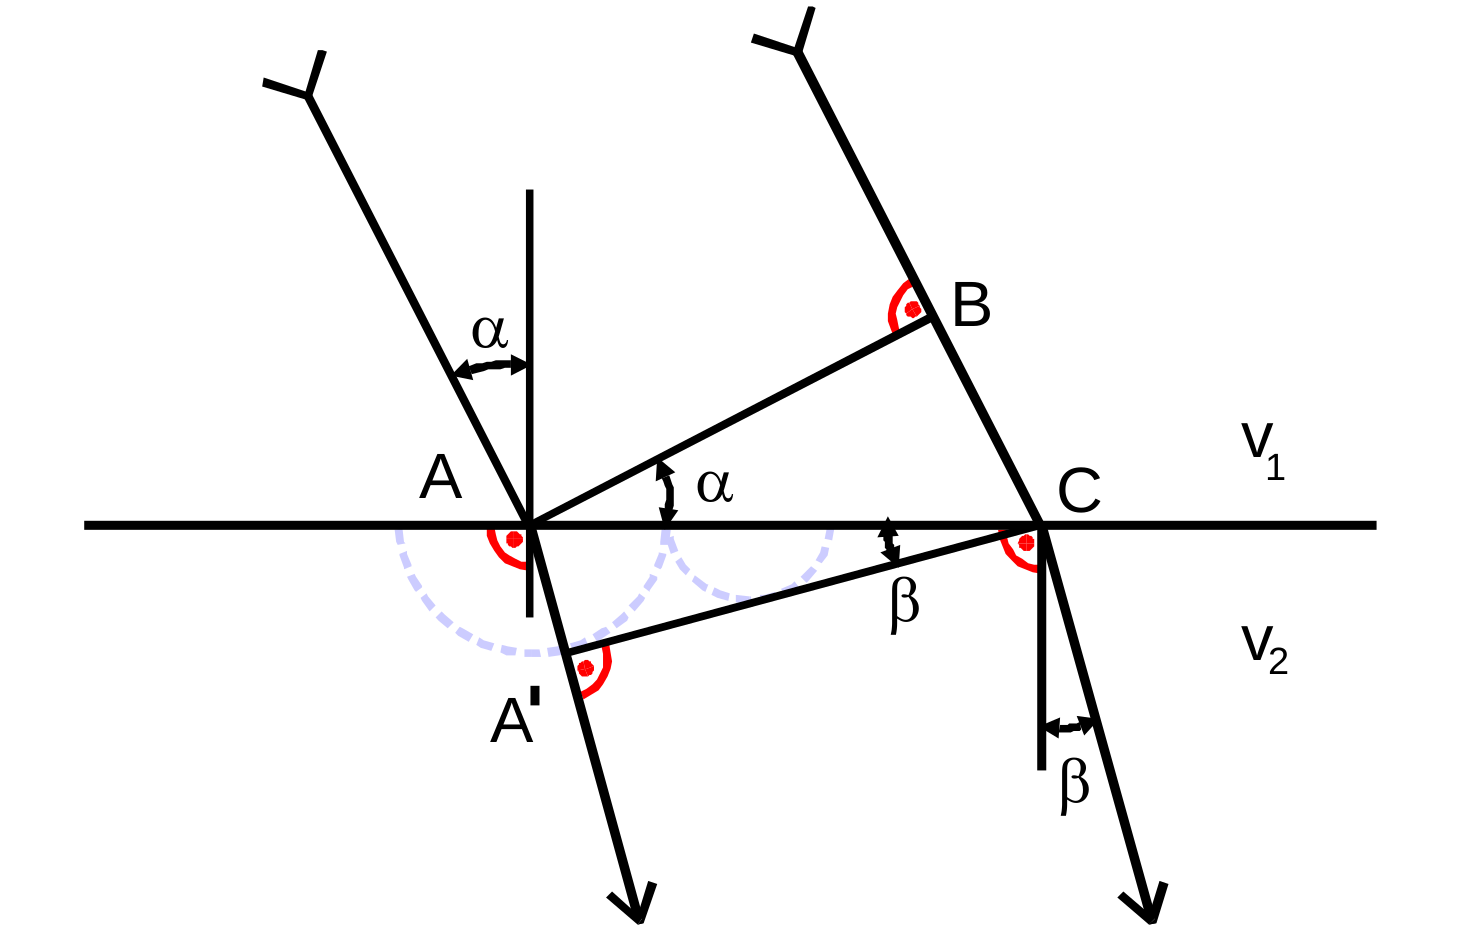
\includegraphics[width=0.6\textheight]{../figures/SBG.png}
  \caption{Veranschaulichung des Strahlengangs mit Hilfe des Huygensschen Prinzips. [Skript V402]}
\label{fig:SBG}
\end{figure}

Wie in Abbildung \ref{fig:SBG} zu sehen ist, trifft die ebene Wellenfront $(\overline{AB})$ im Punkt A schneller auf die Grenzfläche, als im Punkt C. In dieser Zeit $(t_1 = \overline{BC} / v_1)$ hat die Elementarwelle die im Punkt A entsteht, sich schon um $r = t_1v_2$ ausgebreitet, während die im Punkt C erst entsteht.
Durch geometrische Überlegungen lässt sich nun die Beziehung

\begin{equation}
  \frac{\sin{\alpha}}{\sin{\beta}} = \frac{v_1}{v_2} = n
\end{equation}

herleiten, die als \emph{Snelliussches Brechungsgesetz} bekannt ist.

\subsection{Ableitung der Dispersionsrelation}
Dispersion ist ein Phänomen, welches die Frequenzabhängigkeit einer physikalischen Größe beschreibt, in der Optik handelt es sich dabei um die Ausbreitungsgeschwindigkeit von Licht in einem Medium. Nach Gleichung \eqref{equ:n} ist somit auch der Brechungsindex eine frequenzabhängige Größe bzw. abhängig von der Wellenlänge $\lambda$ des Lichtes
\begin{equation}
    n = f(\lambda) \; .
\end{equation}
Dabei handelt es sich um die Dispersionsgleichung, die sich aus der Maxwellschen Theorie elektromagnetischer Wellen ergibt. Dies lässt sich allerdings nur anwenden, wenn die Materie nicht mehr als Kontinuum betrachtet wird, sondern als Ansammlung elektrisch geladener Teilchen, wie Elektronen und Ionenrümpfe. Die Ionenrümpfe können aber für diese Betrachtung vernachlässigt werden, da sichtbares Licht betrachtet wird und diese Wechselwirkung erst bei größeren Wellenlängen eine signifikante Auswirkung hat.

Trifft Licht auf Materie werden die Elektronen durch das elektrische Feld
der Lichtwelle aus ihrer Gleichgewichtslage ausgelenkt. Durch das Wechselfeld wirkt daher eine periodische Kraft auf die Ladungen und führt zu einer erwzungenen Schwingung. Dabei treten auch Resonanzerscheinungen auf, an denen die Materie erkennbar Energie der Lichtwelle absorbiert. Diese klassische Betrachtungsweise reicht aber nicht vollkommen aus um die Wechselwirkung von Licht mit Materie zu beschreiben, dafür wird die Quantentheorie benötigt. Um das zu vermeiden werden in diesem Versuch nur Wellenlängen betrachtet, die genug von den Resonanzstellen entfernt sind, damit die Absorption vernachlässigbar klein wird. Das ist zum Beispiel bei sichtbarem Licht das auf Glas trifft gegeben.

Das Magnetfeld der Lichtwelle erzeugt eine Lorentzkraft, welche die geladenen Teilchen aus ihrer Gleichgewichtslage verschiebt und damit einen elektrischen Dipol erzeugt. Die Polarisation des Mediums ist durch
\begin{equation}
  \vec P = \sum_{h} \vec P_h = \sum_{h} N_h q_h \vec x_h
  \label{equ:P}
\end{equation}
gegeben, mit den Ladungsträgern $q_h$, der Anzahl dieser Ladungsträger pro Volumeneinheit $N_h$, der Auslenkung aus der Gleichgewichtslage $\vec x_h$, während $h$ die unterschiedlichen Teilchenarten bezeichnet.

Eine Auslenkung aus der Gleichgewichtslage erzeugt eine dazu proportionale rücktreibende Kraft. Hinzu kommt eine Dämpfung auf Grund der periodischen Bewegung im elektromagnetischen Feld, die als \emph{"Reibungskraft"} proportional zur Geschwindigkeit der Teilchen sein soll.

Für die Bewegung der Teilchen ergibt sich daraus eine Differentialgleichung der Art
\begin{equation}
  m_h \frac{\mathrm d^2 \vec{x_h}}{\mathrm dt^2} + f_h \frac{\mathrm d \vec{x_h}}{\mathrm dt } + a_h \vec{x_h} = q_h \vec E_0 e^{i \omega t}
  \label{equ:DGL}
\end{equation}
mit den Ladungsträgern $q_h$ und der Teilchenmasse $m_h$. Die Lösung einer solchen Differentialgleichung ist bekannt. Mit Hilfe der Polarisation aus Gleichung \eqref{equ:P} und der \emph{Maxwellschen Relation}
\begin{equation}
  n^2 = \epsilon
  \label{equ:MaxwellRel}
\end{equation}
ergibt sich nach einigen Umformungsschritten der gesuchte Ausdruck für den Brechungsindex in Abhängigkeit der Frequenz des Lichts
\begin{equation}
  \tilde n^2 = 1 + \sum_{h} \frac{1}{\omega_h^2 - \omega^2 + \mathrm{i}\omega \frac{f_h}{m_h}}\frac{N_h q_h^2}{m_h \epsilon_0} \; .
  \label{equ:nkomplex}
\end{equation}
Der Brechungsindex $\tilde n$ ist komplex und kann folglich als
\begin{equation}
  \tilde n = n (1 - \mathrm{i}k)
  \label{equ:nkomplex2}
\end{equation}
mit dem in Gleichung \eqref{equ:n} beschriebenen reellen Brechungsindex $n$ und der Absorptionskonstanten $k$ geschrieben werden. Für die Brechung ist vor allem der Realteil von $\tilde n$ von Interesse. Da die Betrachtung ausreichend weit von den Resonanzstellen entfernt sein soll, wird die Aborption vernachlässigbar klein und damit ist
\begin{equation}
  n^2k \approx 0 \; .
  \label{equ:Naeherung}
\end{equation}
Anschaulich ist die betrachtete Materie damit praktisch farblos und durchsichtig bei den beobachteten Wellenlängen.
Da die Frequenz $\omega$ nicht gemessen werden kann, wird sie durch die Wellenlänge im Vakuum $\lambda$ ersetzt. Daraus ergibt sich für den Brechungsindex
\begin{equation}
  n^2(\lambda) = 1 + \sum_h \frac{N_h q_h^2}{4 \pi^2 c^2 \epsilon_0 m_h}\frac{\lambda^2\lambda_h^2}{\lambda^2 - \lambda_h^2} \; .
  \label{equ:nlambda}
\end{equation}

An dieser Stelle ist nun eine Fallunterscheidung notwendig: Es wird davon ausgegangen, dass das Medium nur eine Absorptionsstelle $\lambda_1$ besitzt. Dann muss zwischen Wellenlängen unterschieden werden, die entweder sehr viel größer oder sehr viel kleiner als $\lambda_1$ sind.

\subsubsection{Wellenlänge $\lambda \gg \lambda_1$}
Werden nur Wellenlängen $\lambda \gg \lambda_1$ betrachtet, kann eine Reihenentwicklung von Gleichung~\eqref{equ:nlambda} nach Potenzen von $\lambda_1/\lambda$ durchgeführt werden. Daraus ergibt sich für den Brechungsindex
\begin{equation}
  n^2(\lambda) = 1 + \frac{N_1 q_1^2 \lambda_1^2}{4 \pi^2 c^2 \epsilon_0 m_1} (1 + (\frac{\lambda_1}{\lambda})^2 + (\frac{\lambda_1}{\lambda})^4 + \cdots )
  \label{equ:taylor1}
\end{equation}
bzw. die \emph{Cauchysche Dispersionsformel}
\begin{align}
  n^2(\lambda) = A_0 + \frac{A_2}{\lambda^2} + \frac{A_4}{\lambda^4} + \cdots
  \label{equ:cauchy}
  \shortintertext{mit}
  A_0, A_2, A_4 > 0 \; .
\end{align}

Der Kurvenverlauf von Gleichung~\eqref{equ:cauchy} ist in Abbildung~\ref{fig:disper1} dargestellt.

\begin{figure}
  \centering
  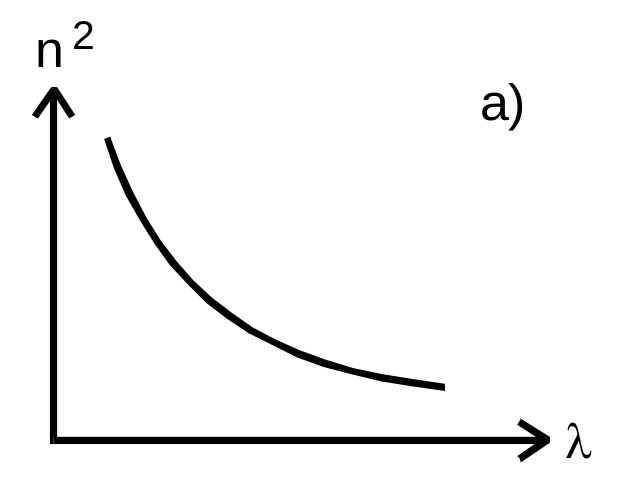
\includegraphics[width=0.4\textheight]{../figures/disper1.png}
  \caption{Dispersionskurve nach der Cauchyschen Dispersionsformel $(\lambda \gg \lambda_1)$. [Skript V402]}
\label{fig:disper1}
\end{figure}

\subsubsection{Wellenlänge $\lambda \ll \lambda_1$}
Jetzt werden Wellenlängen mit $\lambda \ll \lambda_1$ betrachtet, die Reihenentwicklung von Gleichung~\eqref{equ:nlambda} ergibt
\begin{equation}
  n^2(\lambda) = 1 - \frac{N_1 q_1^2 }{4 \pi^2 c^2 \epsilon_0 m_1} (\lambda^2 + (\frac{\lambda^4}{\lambda_1^2}) + (\frac{\lambda^6}{\lambda_1^4}) + \cdots )
  \label{equ:taylor2}
\end{equation}
bzw.
\begin{align}
  n^2(\lambda) = A_0 - A_2'\lambda^2 - A_4'\lambda^4 - \cdots
  \label{equ:disper2}
  \shortintertext{mit}
  A_i' > 0 \text{ für } \mathrm{i} \ge 2 \; .
\end{align}

Die grafische Darstellung des Kurvenverlaufs aus Gleichung~\eqref{equ:disper2} ist in Abbildung~\ref{fig:disper2} dargestellt.

\begin{figure}
  \centering
  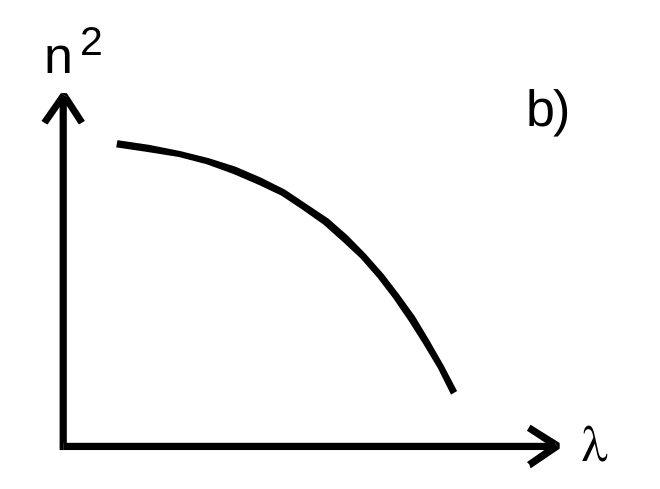
\includegraphics[width=0.4\textheight]{../figures/disper2.png}
  \caption{Dispersionskurve nach Gleichung~\eqref{equ:disper2} mit $\lambda \ll \lambda_1$. [Skript V402]}
\label{fig:disper2}
\end{figure}


Für beide Fälle ergeben sich demnach unterschiedliche Kurvenverläufe (mit unterschiedlicher Krümmung -- zu sehen in Abbildung~\ref{fig:disper1} und \ref{fig:disper2} ), aber in beiden Kurven nimmt der Brechungsindex mit zunehmender Wellenlänge ab (\emph{normale Dispersion}). Um herauszufinden, welche Dispersiongleichung das Material am besten beschreibt, werden einfach die Messdaten mit den Kurvenverläufen verglichen.






%the end

\clearpage
\newpage
\section{Fehlerrechnung}
Im folgenden Kapitel werden die wichtigsten Formeln der Fehlerechnung aufgelistet, welche für die folgende Versuchsauswertung benötigt werden.
Der Mittelwert berechnet sich zu
\begin{equation}
  \overline{x} = \frac{1}{N} \sum_{i=1}^Nx_i
\end{equation}
Der Fehler des Mittelwertes berechnet sich zu
\begin{equation}
  \label{eq:std_mean}
  \Delta \overline{x} = \sqrt{\frac{1}{N(N-1)}\sum_{i=1}^N(x_i-\overline{x})^2}  \; .
\end{equation}
Die Schätzung der Standardabweichung berechnet sich zu
\begin{equation}
  \label{eq:std}
  \Delta x = \sqrt{\frac{1}{N-1}\sum_{i=1}^N(x_i-\overline{x})^2}     \; .
\end{equation}

Für die Fehlerrechnung wird bei allen folgenden Rechnungen das Gaußsche Fehlerfortpflanzungsgesetz
\begin{equation}
\increment{f} = \sqrt{\Bigl(\frac{\partial f}{\partial x_1}\increment{x_1}\Bigr)^2 + \Bigl(\frac{\partial f}{\partial x_2}\increment{x_2}\Bigr)^2 + \dotsc + \Bigl(\frac{\partial f}{\partial x_n}\increment{x_n}\Bigr)^2} 
\end{equation}
für eine Funktion $f(x_1,x_2, \dotsc ,x_n)$, bei der die Größen $x_1, x_2, \dotsc , x_n$ voneinander unabhängig sind, verwendet.

Bei der linearen Regressionsrechnung gilt mit den Parametern $m$ und $b$ und der Ausgleichsgerade $y=mx+b$ der Zusammenhang:
\begin{align}
  m &= \frac{\overline{xy}-\overline{x}\cdot\overline{y}}{\overline{x²} - \overline{x}²} & &  b = \overline{y} - m \overline{x}  \; .
\end{align}
Dabei sind $x_i$ und $y_i$ linear abhängige Messgrößen. Der Fehler dieser Parameter errechnet sich zudem zu
\begin{align}
  \sigma_m^2 &= \frac{\sigma^2}{n(\overline{x²} - \overline{x}²)} & &\sigma_b^2 = \frac{\sigma^2\overline{x²}}{n(\overline{x²} - \overline{x}²)}
\end{align}
% Wenn Messdaten mit Vorhersagen verglichen werden sollen, benutzt man häufig die \emph{root mean square deviation}. Diese ist gegeben durch
% \begin{equation}
%   \label{eq:RMSE}
%   \textrm{RMSD} = \sqrt{\overline{(Y_\textrm{Messung}-Y_\textrm{Vorhersage})^2}}  \; .
% \end{equation}

\clearpage
\newpage
\section{Versuchsaufbau}
\label{sec:Versuchaufbau}
Der Aufbau besteht aus einem geschlossenen Rohrsystem, das mit einer Dopplerphantomflüssigkeit befüllt ist. Das Rohrsystem ist in drei Abschnitte mit unterschiedlichen Rohrinnendurchmessern unterteilt. Um die Flüssigkeit in Bewegung zu setzen ist eine Pumpe angeschlossen, an der seitlich durch ein Regler die Geschwindigkeit in Prozent eingestellt wird. Für die Erzeugung des Ultraschalls wird ein Ultraschall Doppler-Generator mit einer $\SI{2}{\mega\hertz}$ Ultraschallsonde verwendet. Mit dem Programm $\emph{Flowview}$ werden die Daten analysiert und graphisch dargestellt. Alle verwendeten Objekte sind in Abbildung \ref{fig:} dargestellt.

\begin{figure}
  \centering
  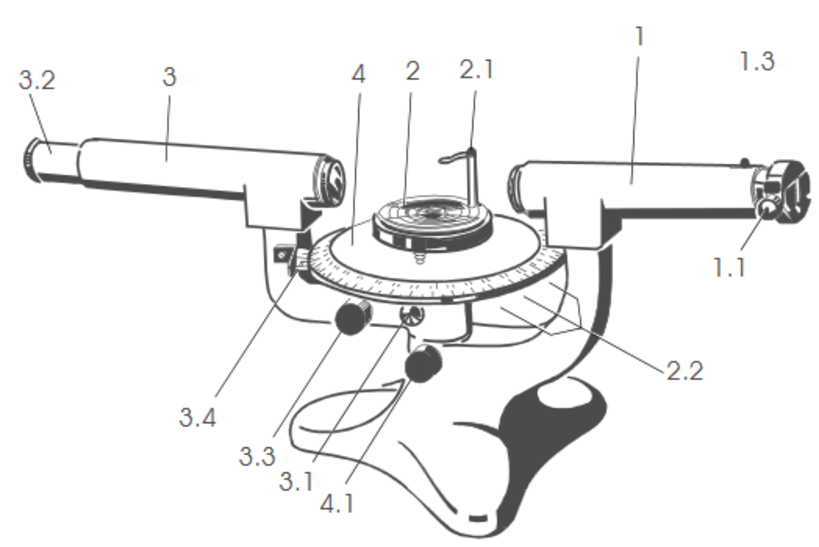
\includegraphics[width=\textwidth]{ressources/Aufbau.pdf}
  \caption{Verwendete Objekte, \cite{skript}.}
  \label{fig:Aufbau}
\end{figure}

Für einen konstanten Winkel $\alpha$ werden Doppler-Prismen mit jeweils drei Einschallwinkeln verwendet, siehe Abbildung $\ref{fig:Prisma}$. Für die jeweiligen Dopplerwinkel gilt
\begin{align}
  \alpha = 90 ^\circ - \arcsin{\left( \sin{(\theta)}\frac{c_\textrm{L}}{c_\textrm{P}}\right)} \;.
  \label{eq:Winkel}
\end{align}

\begin{figure}
  \centering
  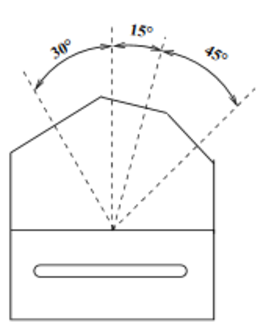
\includegraphics{ressources/Prisma.pdf}
  \caption{Prisma mit drei verschiedenen Winkeln $\Theta$, \cite{skript}.}
  \label{fig:Prisma}
\end{figure}

\clearpage
\newpage
\section{Durchführung}
\label{sec:Durchführung}
Um die Rohdaten des Detektors verwerten zu können, muss zunächst eine Kalibrierung stattfinden. Dazu wird ein Strahler mit bekannten Photonenenergien benötigt. Es wird \ce{^{152} Eu} verwendet, da dieses Material gleich mehrere verschiedene Linien zeigt. Ziel ist es, die Zuordnung zwischen Kanalnummer und Energiewert herauszufinden. Ferner wird diese Messung auch dazu benötigt, um die Effizienz des Detektors zu bestimmen (siehe Kapitel \ref{sec:effizienz}). Für alle Messungen wird eine Zeit von ca. einer Stunde angesetzt. Prinzipiell sind lange Messungen sinnvoll, um dem statistischen Charakter der $\gamma$-Strahlung sowie deren Detektion Rechnung zu tragen.\\
Des weiteren werden die Spektren von \ce{^{137} Cs}, \ce{^{133} Ba} sowie das Spektrum eines unbekannten Steines aufgenommen.

\clearpage
\newpage
\section{Auswertung}
\label{sec:Auswertung}
Die im Folgenden durchgeführten Ausgleichsrechnung wird mit der \emph{curve fit} Funktion aus dem für \emph{Python} geschriebenen package \emph{NumPy}\cite{scipy} durchgeführt. Fehlerrechnungen werden mit dem für \emph{Python} geschriebenen package \emph{Uncertainties}\cite{uncertainties} ausgeführt.

Zunächst soll die Charakteristik, das heißt die Plateausteigung, des Geiger-Müller-Zählrohrs bestimmt werden. Die zu diesem Zwecke aufgenommenen Messdaten sind in Tabelle \ref{table:a} aufgelistet. Für die poissonverteilten Messwerte für die Anzahl der detektierten Impulse $Z$ gilt
\begin{equation}
  \delta Z = \sqrt{Z} \; .
\end{equation}
Zusätzlich in die Tabelle eingetragen sind die abgeleiteten Größen der pro Teilchen freigesetzten Ladungsmenge $\Delta Q$ sowie die Zählrate $N$. Die Ladungsmenge ergibt sich dabei direkt aus Gleichung \eqref{eq:Strom2}, während die Zählrate gemäß
\begin{equation}
  N = \frac{Z}{\Delta t}
\end{equation}
gegeben ist. Für beide Berechnungen ist die im Versuch eingestellte Messzeit $\Delta t = \SI{10}{\second}$ einzusetzen. Die so gewonnen Werte für die Zählrate sind in Abbildung \ref{fig:plot} gegen die Betriebsspannung des Zählrohrs aufgetragen.
\input{build/Tabelle_a_texformat}
\begin{figure}
  \centering
  \includegraphics{build/aufgabenteil_a_plot.pdf}
  \caption{Charakteristik des Zählrohrs. Die für den Plateaubereich ausgewählten Messwerte sind blau gezeichnet.}
  \label{fig:plot}
\end{figure}
Zusätzlich eingezeichnet ist eine Regressionsgerade der Form
\begin{equation*}
  N(U) = aU +b \; ,
\end{equation*}
welche die in blau eingezeichneten, für den Plateaubereich ausgewählten Messwerte berücksichtigt. Hierbei ergibt sich
\begin{align*}
    a &= \input{build/parameter_a.tex} \\
    b &= \input{build/parameter_b.tex} \; .
\end{align*}
Die Plateausteigung $s$ entspricht zwar dem Parameter $a$, jedoch wird sie zumeist in $\%/100\si{\volt}$ angegeben. Der Prozentwert soll sich dabei auf den Funktionswert in der Mitte des Plateaus $N (500\si{\volt}) = \input{build/plateaumitte.tex}$ beziehen. Dann ist
\begin{align*}
  s &= \input{build/plateausteigung.tex}(100\si{\volt})^{-1} \; .
\end{align*}
Die Länge des Plateaus wird vergleichsweise willkürlich mit
\begin{equation*}
  L = ((650-350)\pm 40)\si{\volt} = 300\pm 40 \si{\volt}
\end{equation*}
abgelesen. Der zugehörige Fehler wird aufgrund der ohnehin schwankenden Messwerte großzügig angesetzt.

Um den Zusammenhang zwischen der am Zählrohrdraht gesammelten Ladung pro eintreffendem Impuls $\Delta Q$ und der Betriebsspannung sichtbar zu machen, sind die Messwerte aus Tabelle \ref{table:a} in der Abbildung \ref{fig:plot2} visualisiert.
\begin{figure}
  \centering
  \includegraphics{build/aufgabenteil_e_plot.pdf}
  \caption{Ladung pro eintreffendem Impuls gegenüber der Betriebsspannung.}
  \label{fig:plot2}
\end{figure}
Damit ist die Charakteristik bestimmt und es verbleiben die Aussagen zu Totzeit und Erholungszeit des Geiger-Müller-Zählrohrs. Die Tabelle \ref{table:c} listet hierzu die am Oszilloskop beobachteten Messwerte auf. Zusätzlich werden die in $\si{\centi\meter}$ gemessenen Daten mit Hilfe des am Oszilloskop eingestellten Skalierungsfaktors in die entsprechenden Zeiten übersetzt.
\input{build/Tabelle_c_texformat}
Es ist anzumerken, dass auch hier ein großzügiger Fehler angenommen wird, vor allem bei der Bestimmung der Erholungszeit. Dies ist durch die in sehr unregelmäßiger Abfolge und Position auf dem Oszilloskop erscheinenden Nachentladungsimpulse zu erklären.
Zum Vergleich wird nun die Totzeit mit Hilfe der Zwei-Quellen-Methode gemäß Gleichung \eqref{eq:T} bestimmt. Das in Kapitel \ref{sec:Totzeit} beschriebene Verfahren liefert die in Tabelle \ref{table:d} zu sehenden Ergebnisse.
\input{build/Tabelle_d_texformat}
Da die wahre Größe der Totzeit nicht bekannt ist, wird der folgende relative Fehler auf den als fehlerfrei angenommenen Mittelwert $\overline{T}$ der Messungen der zwei verschiedenen Methoden bezogen.
\begin{align*}
  \epsilon_\text{Tot} = \frac{T_\text{Oszi} - T_\text{2-Quell}} {\overline{T}} = \input{build/RelFehler.tex}
\end{align*}

% Sämtliche im Folgenden durchgeführten Ausgleichsrechnungen werden mit der \emph{curve fit} Funktion aus dem für \emph{Python} geschriebenen package \emph{NumPy}\cite{scipy} durchgeführt. Fehlerrechnungen werden mit dem für \emph{Python} geschriebenen package \emph{Uncertainties}\cite{uncertainties} ausgeführt.

% % Examples
% \begin{equation}
%   U(t) = a \sin(b t + c) + d
% \end{equation}
%
% \begin{align}
%   a &= \input{build/a.tex} \\
%   b &= \input{build/b.tex} \\
%   c &= \input{build/c.tex} \\
%   d &= \input{build/d.tex} .
% \end{align}
% Die Messdaten und das Ergebnis des Fits sind in Abbildung~\ref{fig:plot} geplottet.
%
% %Tabelle mit Messdaten
% \begin{table}
%   \centering
%   \caption{Messdaten.}
%   \label{tab:data}
%   \sisetup{parse-numbers=false}
%   \begin{tabular}{
% % format 1.3 bedeutet eine Stelle vorm Komma, 3 danach
%     S[table-format=1.3]
%     S[table-format=-1.2]
%     @{${}\pm{}$}
%     S[table-format=1.2]
%     @{\hspace*{3em}\hspace*{\tabcolsep}}
%     S[table-format=1.3]
%     S[table-format=-1.2]
%     @{${}\pm{}$}
%     S[table-format=1.2]
%   }
%     \toprule
%     {$t \:/\: \si{\milli\second}$} & \multicolumn{2}{c}{$U \:/\: \si{\kilo\volt}$\hspace*{3em}} &
%     {$t \:/\: \si{\milli\second}$} & \multicolumn{2}{c}{$U \:/\: \si{\kilo\volt}$} \\
%     \midrule
%     1.7 & 10 \\
2.3 & 20 \\
3.5 & 30 \\
4.4 & 40 \\

%     \bottomrule
%   \end{tabular}
% \end{table}
%
% % Standard Plot
% \begin{figure}
%   \centering
%   \includegraphics{build/plot.pdf}
%   \caption{Messdaten und Fitergebnis.}
%   \label{fig:plot}
% \end{figure}
%
% 2x2 Plot
% \begin{figure*}
%     \centering
%     \begin{subfigure}[b]{0.475\textwidth}
%         \centering
%         \includegraphics[width=\textwidth]{Abbildungen/Schaltung1.pdf}
%         \caption[]%
%         {{\small Schaltung 1.}}
%         \label{fig:Schaltung1}
%     \end{subfigure}
%     \hfill
%     \begin{subfigure}[b]{0.475\textwidth}
%         \centering
%         \includegraphics[width=\textwidth]{Abbildungen/Schaltung2.pdf}
%         \caption[]%
%         {{\small Schaltung 2.}}
%         \label{fig:Schaltung2}
%     \end{subfigure}
%     \vskip\baselineskip
%     \begin{subfigure}[b]{0.475\textwidth}
%         \centering
%         \includegraphics[width=\textwidth]{Abbildungen/Schaltung4.pdf}    % Zahlen vertauscht ... -.-
%         \caption[]%
%         {{\small Schaltung 3.}}
%         \label{fig:Schaltung3}
%     \end{subfigure}
%     \quad
%     \begin{subfigure}[b]{0.475\textwidth}
%         \centering
%         \includegraphics[width=\textwidth]{Abbildungen/Schaltung3.pdf}
%         \caption[]%
%         {{\small Schaltung 4.}}
%         \label{fig:Schaltung4}
%     \end{subfigure}
%     \caption[]
%     {Ersatzschaltbilder der verschiedenen Teilaufgaben.}
%     \label{fig:Schaltungen}
% \end{figure*}

\clearpage
\newpage
\section{Diskussion}
\label{sec:Diskussion}

Die ermittelte Ionisationsenergie des Quecksilbers,
\begin{align*}
  E_{\text{Ion}} &= \input{build/c_ion.tex},
\end{align*}
weist im Vergleich zum Literaturwert \cite{ionisationsenergie},
\begin{align*}
  E_{\text{Ion, Lit}} &= \SI{10.438}{\electronvolt},
\end{align*}
eine relative Abweichung von
\begin{align*}
  E_{\text{Ion,rel}} &= \input{build/c_ion_rel_err.tex}
\end{align*}
auf.
Dies ist ein Indiz dafür, dass das bestimmte Kontaktpotential von etwa
\begin{align*}
  K &= \SI{3.1}{\volt}
\end{align*}
zutreffend ist.\\
Im Bezug zur aufgenommenen Franck-Hertz-Kurve stellt sich die Frage, welche Ursache der unerwartete Verlauf nach dem vierten Maximum hat.
Da Aufnahmen bei verschiedenen Temperaturen zum gleichen Phänomen führten, liegt die Ursache vermutlich in einem systematischen Fehler des Aufbaus noch ungeklärter Herkunft.
Die eindeutig messbaren Maxima, sowie deren Abstände,
\begin{align*}
  \Delta U &= \input{build/b_U_max_delta.tex},
\end{align*}
kommen dem Literaturwert \cite{anregungsenergie},
\begin{align*}
  \Delta U_{\text{Lit}} &= \SI{4,9}{\electronvolt},
\end{align*}
mit einer relativen Abweichung von
\begin{align*}
  \Delta U_{\text{rel}} &= \input{build/b_anregung_rel.tex}
\end{align*}
sehr nahe.
Die elastischen Stöße, selbst wenn sie zentral sind, sind doch statistisch gleichmäßig verteilt und sorgen demnach nur für eine Verbreiterung der Peaks.
Daher können sie vernachlässigt werden.\\
Insgesamt unterstützt der Versuch eine quantenmechanische Sichtweise auf die Elektronenhülle, zumindest bei Quecksilberatomen.

\clearpage
\newpage

\printbibliography

\clearpage
\newpage
\begin{appendix}
\section{Messdaten}
\centering
\begin{figure}
\includepdf[width=0.9\textwidth, pages={1}]{ressources/Messdaten.pdf}
\end{figure}
\newpage
\input{build/Tabelle_messdaten_texformat.tex}
\end{appendix}

\section{Anhang}

\begin{figure}[H]
  \centering
  \includegraphics[height=14cm]{messdaten/daten-1.jpg}
  \caption{Originaldaten Teil 1.}
  \label{fig:original1}
\end{figure}

\begin{figure}[H]
  \centering
  \includegraphics[height=14cm]{messdaten/daten-2.jpg}
  \caption{Originaldaten Teil 2.}
  \label{fig:original2}
\end{figure}

\begin{figure}[H]
  \centering
  \includegraphics[height=14cm]{messdaten/daten-3.jpg}
  \caption{Originaldaten Teil 3.}
  \label{fig:original2}
\end{figure}


\end{document}


% % Examples
% \begin{equation}
%   U(t) = a \sin(b t + c) + d
% \end{equation}
%
% \begin{align}
%   a &= \input{a.tex} \\
%   b &= \input{b.tex} \\
%   c &= \input{c.tex} \\
%   d &= \input{d.tex} .
% \end{align}
% Die Messdaten und das Ergebnis des Fits sind in Abbildung~\ref{fig:plot} geplottet.
%
% %Tabelle mit Messdaten
% \begin{table}
%   \centering
%   \caption{Messdaten.}
%   \label{tab:data}
%   \sisetup{parse-numbers=false}
%   \begin{tabular}{
%     S[table-format=1.3]
%     S[table-format=-1.2]
%     @{${}\pm{}$}
%     S[table-format=1.2]
%     @{\hspace*{3em}\hspace*{\tabcolsep}}
%     S[table-format=1.3]
%     S[table-format=-1.2]
%     @{${}\pm{}$}
%     S[table-format=1.2]
%   }
%     \toprule
%     {$t \:/\: \si{\milli\second}$} & \multicolumn{2}{c}{$U \:/\: \si{\kilo\volt}$\hspace*{3em}} &
%     {$t \:/\: \si{\milli\second}$} & \multicolumn{2}{c}{$U \:/\: \si{\kilo\volt}$} \\
%     \midrule
%     1.7 & 10 \\
2.3 & 20 \\
3.5 & 30 \\
4.4 & 40 \\

%     \bottomrule
%   \end{tabular}
% \end{table}
%
% % Standard Plot
% \begin{figure}
%   \centering
%   \includegraphics{plot.pdf}
%   \caption{Messdaten und Fitergebnis.}
%   \label{fig:plot}
% \end{figure}
